% SEDS500 Project Defense Presentation
% Privacy-Preserving Synthetic Tabular Data Generation Using Diffusion Models
% Author: Umut Akın
% Date: January 2026

\documentclass[aspectratio=169,11pt]{beamer}

% Theme - Dracula
\usetheme{Madrid}
\usecolortheme{default}

% Dracula color palette
\definecolor{draculabg}{RGB}{40, 42, 54}
\definecolor{draculacurrent}{RGB}{68, 71, 90}
\definecolor{draculafg}{RGB}{248, 248, 242}
\definecolor{draculacomment}{RGB}{98, 114, 164}
\definecolor{draculacyan}{RGB}{139, 233, 253}
\definecolor{draculagreen}{RGB}{80, 250, 123}
\definecolor{draculaorange}{RGB}{255, 184, 108}
\definecolor{draculapink}{RGB}{255, 121, 198}
\definecolor{draculapurple}{RGB}{189, 147, 249}
\definecolor{draculared}{RGB}{255, 85, 85}
\definecolor{draculayellow}{RGB}{241, 250, 140}

% Apply Dracula theme
\setbeamercolor{background canvas}{bg=draculabg}
\setbeamercolor{normal text}{fg=draculafg}
\setbeamercolor{structure}{fg=draculapurple}
\setbeamercolor{frametitle}{bg=draculacurrent,fg=draculafg}
\setbeamercolor{title}{fg=draculafg}
\setbeamercolor{subtitle}{fg=draculacyan}
\setbeamercolor{title separator}{fg=draculapurple}
\setbeamercolor{palette primary}{bg=draculacurrent,fg=draculafg}
\setbeamercolor{palette secondary}{bg=draculacurrent,fg=draculafg}
\setbeamercolor{palette tertiary}{bg=draculapurple,fg=draculafg}
\setbeamercolor{palette quaternary}{bg=draculacurrent,fg=draculafg}
\setbeamercolor{titlelike}{parent=palette primary,fg=draculafg}
\setbeamercolor{author}{fg=draculafg}
\setbeamercolor{institute}{fg=draculacomment}
\setbeamercolor{date}{fg=draculacomment}
\setbeamercolor{item}{fg=draculacyan}
\setbeamercolor{block title}{bg=draculacurrent,fg=draculagreen}
\setbeamercolor{block body}{bg=draculabg,fg=draculafg}
\setbeamercolor{block title alerted}{bg=draculared,fg=draculafg}
\setbeamercolor{block body alerted}{bg=draculacurrent,fg=draculafg}
\setbeamercolor{alerted text}{fg=draculared}
\setbeamercolor{footline}{fg=draculacomment}
\setbeamercolor{section in toc}{fg=draculacyan}
\setbeamercolor{subsection in toc}{fg=draculafg}
\setbeamercolor{section number projected}{bg=draculapurple,fg=draculafg}
\setbeamercolor{subsection number projected}{bg=draculacurrent,fg=draculafg}

% Packages
\usepackage[utf8]{inputenc}
\usepackage[T1]{fontenc}
\usepackage{graphicx}
\usepackage{booktabs}
\usepackage{amsmath}
\usepackage{tikz}
\usepackage{colortbl}

% Table colors for dark theme
\arrayrulecolor{draculacomment}

% Graphics path
\graphicspath{{../figures/}}

% Remove navigation symbols
\setbeamertemplate{navigation symbols}{}

% Add slide numbers
\setbeamertemplate{footline}[frame number]

% Title information
\title[Synthetic Data via Diffusion]{Privacy-Preserving Synthetic Tabular Data Generation Using Diffusion Models}
\subtitle{SEDS500 Graduation Project}
\author{Umut Ak{\i}n}
\institute[IZTECH]{
    Izmir Institute of Technology\\
    Graduate School of Engineering and Sciences\\
    Department of Computer Engineering
}
\date{January 2026}

\begin{document}

% Title slide
\begin{frame}
    \titlepage
\end{frame}

%===============================================
\section{Abstract}
%===============================================

\begin{frame}{Abstract}
    \begin{block}{Research Summary}
        This project investigates \textbf{diffusion models} as a privacy-preserving approach for generating synthetic tabular data.
    \end{block}

    \vspace{0.3cm}
    \textbf{Method:} TabDDPM-style diffusion with hybrid Gaussian-Multinomial noise

    \vspace{0.3cm}
    \textbf{Comparison:} Against CTGAN (GAN-based) and SMOGN (interpolation-based)

    \vspace{0.3cm}
    \textbf{Key Results:}
    \begin{itemize}
        \item \textbf{87--98\%} of baseline model performance with synthetic data alone
        \item Significantly outperforms CTGAN (35\%) and SMOGN (fails completely)
        \item \textbf{Zero privacy leakage} (membership inference AUC = 0.51)
    \end{itemize}

    \vspace{0.3cm}
    \textbf{Conclusion:} Diffusion models are superior for generating high-utility, privacy-preserving synthetic tabular data.
\end{frame}

%===============================================
\section{Introduction}
%===============================================

\begin{frame}{Motivation \& Problem Definition}
    \begin{columns}
        \column{0.5\textwidth}
        \textbf{The Challenge:}
        \begin{itemize}
            \item Organizations need to share data for ML collaboration
            \item Privacy regulations (GDPR, KVKK) restrict data sharing
            \item Traditional methods (GANs, interpolation) struggle with mixed data types
        \end{itemize}

        \vspace{0.4cm}
        \begin{block}{Research Question}
            Do diffusion models produce more realistic synthetic tabular data than traditional methods?
        \end{block}

        \column{0.5\textwidth}
        \centering
        \textbf{Solution: Synthetic Data}

        \vspace{0.2cm}
        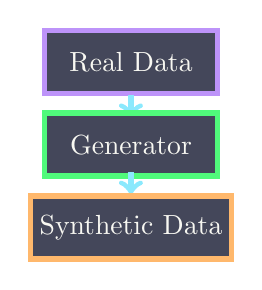
\begin{tikzpicture}[scale=0.7]
            \node[draw=draculapurple, line width=2pt, rectangle, fill=draculacurrent, text=draculafg, minimum width=2.2cm, minimum height=0.8cm] at (0,1.5) {Real Data};
            \draw[->, line width=2pt, draculacyan] (0,0.9) -- (0,0.5);
            \node[draw=draculagreen, line width=2pt, rectangle, fill=draculacurrent, text=draculafg, minimum width=2.2cm, minimum height=0.8cm] at (0,0) {Generator};
            \draw[->, line width=2pt, draculacyan] (0,-0.5) -- (0,-0.9);
            \node[draw=draculaorange, line width=2pt, rectangle, fill=draculacurrent, text=draculafg, minimum width=2.2cm, minimum height=0.8cm] at (0,-1.5) {Synthetic Data};
        \end{tikzpicture}

        \vspace{0.3cm}
        \textbf{Evaluation Criteria:}
        \begin{enumerate}
            \item \textbf{Utility}: ML performance on real data
            \item \textbf{Privacy}: No information leakage
        \end{enumerate}
    \end{columns}
\end{frame}

\begin{frame}{Proposed Solution}
    \begin{center}
    \tikz{
        \node[fill=draculapurple, rounded corners=5pt, inner sep=10pt, text=draculafg] {
            \large\textbf{Implement TabDDPM-style diffusion for tabular data generation}
        };
    }
    \end{center}

    \vspace{0.3cm}
    \begin{columns}[t]
        \column{0.5\textwidth}
        \textbf{Key innovations:}
        \begin{itemize}
            \item Hybrid noise handling
            \item Gaussian for numerical features
            \item Multinomial for categorical features
            \item Log-space operations for stability
            \item KL divergence loss
        \end{itemize}

        \column{0.5\textwidth}
        \textbf{Methods compared:}
        \begin{itemize}
            \item \textbf{TabDDPM-style} (ours)
            \item CTGAN (GAN-based)
            \item SMOGN (interpolation)
        \end{itemize}

        \vspace{0.3cm}
        \textbf{Datasets:}
        \begin{itemize}
            \item Production (5,370 samples)
            \item Ozel Rich (2,670 samples)
        \end{itemize}
    \end{columns}
\end{frame}

%===============================================
\section{Related Research}
%===============================================

\begin{frame}{Related Research}
    \begin{table}
        \centering
        \small
        \begin{tabular}{llll}
            \toprule
            \textbf{Paper} & \textbf{Venue} & \textbf{Approach} & \textbf{Key Innovation} \\
            \midrule
            TabDDPM & ICML 2023 & Diffusion & Hybrid Gaussian-Multinomial noise \\
            CTGAN & NeurIPS 2019 & GAN & Mode-specific normalization \\
            STaSy & ICLR 2023 & Score-based & Self-paced learning \\
            TabSyn & ICLR 2024 & Latent diffusion & Transformer VAE encoder \\
            \bottomrule
        \end{tabular}
    \end{table}

    \vspace{0.3cm}
    \textbf{Why diffusion over GANs?}
    \begin{itemize}
        \item GANs suffer from mode collapse and training instability
        \item Diffusion models have stable training dynamics
        \item Iterative refinement captures full data distribution
    \end{itemize}

    \vspace{0.3cm}
    \textbf{Our contribution:} Implement and evaluate TabDDPM-style diffusion on real organizational datasets with privacy validation.
\end{frame}

%===============================================
\section{Solution Approach}
%===============================================

\begin{frame}{Solution: TabDDPM Diffusion Model}
    \begin{columns}
        \column{0.5\textwidth}
        \textbf{How Diffusion Works:}
        \begin{itemize}
            \item \textbf{Forward}: Gradually add noise ($T$=1000 steps)
            \item \textbf{Reverse}: Learn to denoise step-by-step
            \item Neural network: noise $\rightarrow$ realistic data
        \end{itemize}

        \vspace{0.3cm}
        \textbf{TabDDPM Hybrid Approach:}
        \begin{itemize}
            \item \textbf{Numerical}: Gaussian diffusion
            \item \textbf{Categorical}: Multinomial diffusion
            \item Process both simultaneously
        \end{itemize}

        \column{0.5\textwidth}
        \centering
        \includegraphics[width=0.95\textwidth]{fig6_diffusion_process.png}

        \vspace{0.2cm}
        \small\textit{Iterative denoising from random noise}
    \end{columns}

    \vspace{0.3cm}
    \begin{block}{Key Advantage}
        Stable training + captures full distribution (no mode collapse like GANs)
    \end{block}
\end{frame}

%===============================================
\section{Validation Approach}
%===============================================

\begin{frame}{Datasets \& Experimental Setup}
    \textbf{Two real-world organizational datasets (Turkish fastener company):}

    \vspace{0.3cm}
    \begin{table}
        \centering
        \begin{tabular}{llrll}
            \toprule
            \textbf{Dataset} & \textbf{Domain} & \textbf{Samples} & \textbf{Features} & \textbf{Target} \\
            \midrule
            Production & Sales quotation & 5,370 & 7 num + 35 cat & Quote amount \\
            Ozel Rich & Custom mfg & 2,670 & 2 num + 4 cat & Machine time \\
            \bottomrule
        \end{tabular}
    \end{table}

    \vspace{0.3cm}
    \textbf{Evaluation scenarios:}
    \begin{enumerate}
        \item \textbf{Replacement}: Train on synthetic only, test on real data
        \item \textbf{Augmentation}: Train on real + synthetic, test on real data
    \end{enumerate}

    \vspace{0.3cm}
    \textbf{Metrics:} R\textsuperscript{2} score (utility), MIA AUC (privacy)
\end{frame}

\begin{frame}{Results: Utility Comparison}
    \begin{columns}
        \column{0.5\textwidth}
        \textbf{Ozel Rich Dataset} (Replacement scenario)
        \begin{table}
            \centering
            \small
            \begin{tabular}{lrr}
                \toprule
                \textbf{Method} & \textbf{R\textsuperscript{2}} & \textbf{\%} \\
                \midrule
                Baseline & 0.645 & 100\% \\
                \midrule
                SMOGN & -0.14 & FAILED \\
                CTGAN & 0.229 & 35.5\% \\
                \textbf{TabDDPM} & \textbf{0.563} & \textbf{87.3\%} \\
                \bottomrule
            \end{tabular}
        \end{table}

        \vspace{0.2cm}
        \textbf{Production Dataset}
        \begin{table}
            \centering
            \small
            \begin{tabular}{lrr}
                \toprule
                \textbf{Scenario} & \textbf{R\textsuperscript{2}} & \textbf{\%} \\
                \midrule
                Replacement & 0.979 & \textbf{98.4\%} \\
                Augmentation & 0.994 & \textbf{100\%} \\
                \bottomrule
            \end{tabular}
        \end{table}

        \column{0.5\textwidth}
        \centering
        \includegraphics[width=0.95\textwidth]{fig4_method_summary.png}

        \vspace{0.3cm}
        \textbf{Key findings:}
        \begin{itemize}
            \item TabDDPM: \textbf{87--98\%} of baseline
            \item CTGAN: 35\% | SMOGN: Failed
            \item Generalizes across datasets
        \end{itemize}
    \end{columns}
\end{frame}

\begin{frame}{Results: Privacy Evaluation}
    \textbf{Membership Inference Attack: Can attacker identify training records?}

    \vspace{0.3cm}
    \begin{columns}
        \column{0.45\textwidth}
        \begin{table}
            \centering
            \begin{tabular}{lrl}
                \toprule
                \textbf{Method} & \textbf{AUC} & \textbf{Status} \\
                \midrule
                Random & 0.50 & -- \\
                \midrule
                TabDDPM & \textbf{0.51} & SAFE \\
                Simple Diff & 0.51 & SAFE \\
                SMOGN & 0.53 & SAFE \\
                \bottomrule
            \end{tabular}
        \end{table}

        \vspace{0.3cm}
        \textbf{AUC $\approx$ 0.5 = Random guessing}\\
        \textbf{= No privacy leakage}

        \column{0.55\textwidth}
        \centering
        \includegraphics[width=\textwidth]{fig8_privacy_comparison.png}
    \end{columns}

    \vspace{0.3cm}
    \begin{block}{Key Result}
        TabDDPM: \textbf{Highest utility} (87--98\%) + \textbf{Excellent privacy} (AUC = 0.51)
    \end{block}
\end{frame}

%===============================================
\section{Conclusion \& Future Work}
%===============================================

\begin{frame}{Conclusion \& Future Work}
    \begin{columns}
        \column{0.55\textwidth}
        \textbf{Key Findings:}
        \begin{itemize}
            \item TabDDPM: \textbf{87--98\%} utility vs 35\% (CTGAN)
            \item Privacy-safe: MIA AUC = 0.51 (random guessing)
            \item SMOGN fails on complex tabular data
            \item Generalizes across different datasets
        \end{itemize}

        \vspace{0.3cm}
        \begin{block}{Main Conclusion}
            \centering
            Diffusion models are superior for\\privacy-preserving synthetic data
        \end{block}

        \column{0.45\textwidth}
        \textbf{Limitations:}
        \begin{itemize}
            \item 2 organizational datasets
            \item Basic privacy evaluation
        \end{itemize}

        \vspace{0.2cm}
        \textbf{Future Work:}
        \begin{itemize}
            \item TabSyn (latent diffusion)
            \item Differential privacy
            \item Public benchmarks
        \end{itemize}

        \vspace{0.2cm}
        \textbf{Applications:}
        \begin{itemize}
            \item Safe data sharing
            \item GDPR/KVKK compliance
        \end{itemize}
    \end{columns}
\end{frame}

\begin{frame}{}
    \centering
    \Huge \textbf{Thank You}

    \vspace{1cm}
    \Large Questions?

    \vspace{1cm}
    \normalsize
    \textbf{Umut Ak{\i}n}\\
    Izmir Institute of Technology\\
    SEDS500 Graduation Project\\
    January 2026
\end{frame}

\end{document}
